\documentclass{article}

% stations weg, heb het alleen over receivers. Een stations is dan ook gewoon een receiver

%% polarisaties weg halen.
%% Wel uitleggen dat ze er zijn, maar voor de filters en de correlator
%% zijn het gewoon onafhankelijke receivers. Dit maakt de pseudo code + optimalisaties veel compacter.
% @@@ Rob: dit klopt helemaal niet. Voor de polarisaties moet je namelijk ALLE combinaties uitrekenen.
% DUS zowel XY als YX. Voor stations doe je dit niet. We kunnen polarisaties dus niet weg laten.
% Daarom kwam John ook op een AI van 0.5 uit IPV 1.





% opencl uitzoeken
%  - hoe gaat opencl om met random writes?


% uitzoeken: andere toepassingen van correleren: geofysica? radar? wifi 802.11n, wimax???



% zoek parallelisme: onafhankelijke berekeningen
% voor de correlator geldt dat de berekiningen onafhankelijk zijn, maar IO niet!
% met many cores is de I/O vaak de bottleneck


%% pas je algorithmen aan op many-cores


%% 1) zoek parallelisme in je algorithme.
%%    vaak aanwezig. Zoek onafhankelijke operaties:
%%     voorbeelden:
%%    - correlator: kanalen, polatisaties, subbanden zijn onafhankelijk.
%%    - polyphase: stations zijn onafhankelijk
%%    - imaging: maak parallelisme: beeld elk kanaal af op een image, tel deze later op

  
%% 2) mem bw/ops neemt af met many cores
%%    optimaliseer.

%% dus optimaliseren: 
%%     - algo specifiek (reduceer mem loads)
%%     - architectuur-specifieke optimalisaties (cache gedrag, delays, floating point instructions)


\usepackage{spconf}
\usepackage{graphicx}
\usepackage{listings}

\title{How to Build a Correlator on Many-Core Hardware}

\name{Rob V. van Nieuwpoort and John W. Romein}

\address{Stichting ASTRON (Netherlands Institute for Radio Astronomy) \\
Oude Hoogeveensedijk 4, 7991 PD\ \ Dwingeloo, The Netherlands \\
\texttt{\{nieuwpoort,romein\}@astron.nl}
}


\begin{document}

\maketitle

\begin{abstract}
\end{abstract}

\section{Introduction}
% wat gaat de lezer leren van dit paper?

% we geven een leidraad voor het kiezen van de juiste architectuur voor het probleem van de lezer
% voor goede performance heb je nodig:
%  - kennis van algorithme
%  - kennis van de architecturen
%  - inzicht over hoe je de mapping van algorithme op architectuur het beste kunt doen
% dit paper geeft inzicht in de verschillen tussen architecturen, en inzicht over welke factoren belangrijk zijn om de mapping goed te doen.

Radio telescopes produce enormous amounts of data.
The stations of the \emph{Low Frequency Array
(LOFAR)\/}~\cite{Butcher:04,deVos:09}, for instance, will produce some tens of
petabits per day; the dishes from the Australian SKA Pathfinder (ASKAP) will
even produce over six exabits per day.
To extract the sky signal from the system noise, the \emph{correlator\/}
correlates the signals by multiplying the samples of each pair of receivers.
Additionally, the correlator integrates correlations over time, to reduce
the amount of data.

Traditionally, custom-built hardware is used to correlate the signals.
A recent development is to use a supercomputer~\cite{Romein:06,Romein:09b}.
Both approaches have important advantages and disadvantages.
Custom-built hardware is efficient and consumes modest amounts of power, but is
inflexible, expensive to design, and has a long development time.
Solutions that use a supercomputer are much more flexible, but are less
efficient, consume more power, and are expensive to purchase and maintain.
Future instruments, like the Square Kilometre Array (SKA), need several orders
of magnitude more computational resources.
It is likely that the requirements of the SKA cannot be met by using
current supercomputer technology.

During the past ten years, the high-performance computing community has
steadily adopted clusters of Graphics Processor Units (GPUs) as a viable
alternative to supercomputers, due to their unparalleled growth in
computational performance, increasing flexibility, increasing programmability,
high power efficiency, and low purchase costs.
High-end GPUs are highly parallel and contain hundreds of processor cores.
%% However, their usefulness is often limited to applications that do not require
%% double-precision floating-point arithmetics, since there is no need for
%% double-precision calculations to play games.
%% Hence, the support for double-precision arithmetic is typically poor.
%% Fortunately, many signal-processing applications do not require double
%% precision.

The IBM Cell Broadband Engine~\cite{Gschwind:06}, well known from the
PlayStation~3, is another example of a processor that combines GPU and CPU
qualities into one design.
The Cell BE consists of an ``ordinary'' PowerPC core and eight powerful
\emph{Synergistic Processing Elements (SPEs)}, co-processors that provide
the bulk of the processing power.
The SPEs are vector processors with fast, local memories, and are capable
of transferring data from and to main memory by means of DMA.
Programming the SPEs requires more effort than programming an ordinary CPU,
but various studies showed that the Cell BE performs very well on
signal-processing tasks like FFTs~\cite{?}.

In this article, we explain how modern multi-core architectures can be
exploited for signal-processing purposes.
Additionally, we give insights into their architectural limitations, and how
to best cope with them.
We treat five different, popular multi-core architectures: the IBM Cell BE,
GPUs from Nvidia and ATI, the IBM Blue Gene/P, and
the Intel Core i7 processors.
We discuss their similarities and differences, and how the architectural
differences affect optimization choices and the eventual performance of a
correlator.
We strongly focus on correlators, but many of the findings, claims, and
optimizations hold for other signal-processing algorithms as well, both in and outside the
area of radio astronomy.
We discuss the programmability of each of the architectures, but this paper
should be of special interest to those who are willing to put some extra
programming effort to obtain good performance, even if high-level programming
support is not available.


In this paper, we use the LOFAR
telescope as an example, but the results apply equally well
to other instruments. 


\section{Trends in radio astronomy}

%- signal processing neemt een dominantere rol (meer antennes, etc)
%- voorbeelden. pathfinders voor SKA. 
%- computationally intensive, SKA even more



During the past decade, new types of radio-telescope concepts emerged that
rely less on concrete, steel, and extreme cooling techniques, but more on
signal-processing techniques.
For example, LOFAR~\cite{Butcher:04,deVos:09} is a distributed sensor network
that combines the signals of tens of thousands of simple receiver elements.
%Unlike traditional telescopes, that typically use custom-built hardware to
%process data, LOFAR uses programmable FPGAs for on-the-field station
%processing and a Blue Gene/P supercomputer to process data centrally, in real
%time.
Also, Aperture Array tiles like Embrace~\cite{?} and Focal Plane Arrays
like Apertif~\cite{?} are novel multi-receiver concepts that require huge
amounts of processing power to combine the data from the receiving elements.
Unlike single-pixel feeds from traditional dish-based telescopes, these
concepts combine the advantages of higher sensitivity, higher resolution,
and multiple, concurrent observation directions.

%@@@ later even kijken: computing advances maken nieuwe signal processing technieken en telescopen / instrumenten mogelijk.



%% @@@
%% It is important that the authors take a tutorial 
%% oriented style and more carefully introduce the 
%% application context, including radio-astronomy 
%% basics, instruments that they use (including 
%% installation roadmap).  The algorithm is quite 
%% simple and so the strength of the paper lies in 
%% the thoroughness of the analysis, and the 
%% aforementioned tutorial background.
%% @@@

%% SKA + pathfinders: EMBRACE, LOFAR, ASKAP, meerKAT





The signal-processing hardware technology used to process telescope data
also changes rapidly.
Only a decade ago, correlators required special-purpose ASICs to keep up with
the high data rates and processing requirements.
The advent of sufficiently fast FPGAs significantly lowered the developments
times and costs of newer-generation correlators, and increased the flexibility
substantially.
LOFAR requires even more flexibility to support many different processing
pipelines for various observation modes, and uses a Blue Gene/P supercomputer
to perform real-time, central processing.

GPUs seem to be a viable complement to the aforementioned processing platforms.
GPUs provide more processing power and are more power-efficient than CPUs,
while GPUs are more flexible and easier to program than FPGAs.
Since GPUs of different vendors are mutually quite different, we did an
extensive performance comparison between the architectures of popular GPUs 
for signal-processing purposes, particularly, for correlation
purposes~\cite{Nieuwpoort:09}.

%@@@ Cell



\section{Correlating signals}



%XF vs FX. lofar is FX. Met een groter aantal inputs is FX efficienter?
%transpose


\begin{figure*}[t]
\begin{center}
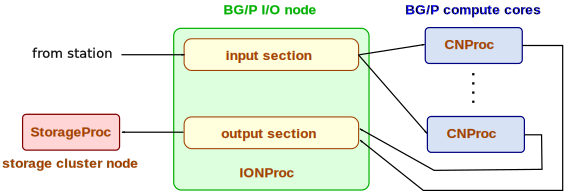
\includegraphics[width=12cm]{figures/processing-overview.pdf}
\end{center}
\vspace{-0.5cm}
\caption{A simplified view of LOFAR processing.}
\label{fig-processing-overview}
\end{figure*}

An overview of the processing needed for the standard imaging pipeline
of LOFAR is shown in Figure~\ref{fig-processing-overview}.  The
thickness of the lines indicates the size of the data streams.  The
data streams from the different receivers must be filtered, delays in
the signal path must be compensated for, and the data streams from
different receivers must be cross-correlated. The correlation process
performs a data reduction by integrating samples over time.  In this
paper, we focus on the correlator step (the gray box in
Figure~\ref{fig-processing-overview}), because it must deal with the full data streams
from all receivers. Moreover, its costs grow
quadratically with the number of receivers, while all other steps have a
lower time complexity.  

The data streams from the receivers contain samples, which are complex
numbers that represent the amplitude and phase of a signal at a
particular time.  The receivers are dual-polarized; they take separate
samples from orthogonal (X and Y) directions.  The LOFAR receivers
support 4, 8 and 16 bit integer samples, where the normal mode of
operation uses the 16 bit samples. The smaller samples are important
for observations that require larger frequency bands (but with less accuracy).
The future SKA telescope will
likely use 2 bit samples.  Before filtering and correlating, the
samples are converted to single precision floating point.  This is
accurate enough for our purposes. From the perspective of the
correlator, samples thus consist of four 32-bit floating point
numbers: two polarizations, each with a real and an imaginary part.

Prior to correlation, an FX correlator must reorder the data that comes from
the receivers:
each input carries the signals of from many frequency subbands from a single
receiver, but the correlator needs data from a single frequency of all inputs.
Depending on the data rate, switching the data can be a real challenge.
The data reordering phase is outside the scope of this paper, but a correlator
implementation cannot ignore this issue.
The LOFAR Blue Gene/P correlator uses the fast 3-D~torus for this purpose;
other multi-core architectures need external switches.

The received signals from sky sources are so weak, that the antennas 
mainly receive noise. To see if there is statistical coherence
in the noise, simultaneous samples of each pair of receivers are correlated, 
by multiplying the sample of one receiver with the complex
conjugate (i.e., the imaginary part is negated) of the sample of the other receiver.
To reduce the output size, the correlations are integrated, by accumulating all products. 
Therefore, the correlator is mostly multiplying and adding complex numbers.
Both polarizations of a station A are correlated with both polarizations 
of a station B, yielding correlations in XX, XY, YX, and YY
directions. Receivers are also autocorrelated, i.e., with
themselves. 
The correlator algorithm itself thus is straightforward, and can be
written in a single formula: \\
$C_{s_1,s_2\geq s_1,p_1\in\{X,Y\},p_2\in\{X,Y\}} = \displaystyle\sum_{t} Z_{s_1,t,p_1} * Z_{s_2,t,p_2}^\ast$ 

The total number of correlations we have to compute is $(nrReceivers \times
(nrReceivers + 1)) / 2$, since we need each pair of correlations only
once. This includes the autocorrelations (the correlation of a receiver with itself),
since we need this later in the pipeline for calibration purposes.
The autocorrelations can be computed with half the number of instructions.

We can implement the correlation operation very efficiently, with only
four fused-multily-add (fma) instructions, doing eight floating-point operations in
total. For each pair of receivers, we have to do this four times, once
for each combination of polarizations. Thus, in total we need 32
operations. To perform these operations, we have to load the samples generated by two different receivers from memory.
As explained above, the samples each consist of four single precision floating point numbers (a real and imaginary part, and two polarizations).
Therefore, we need to load 8 floats or 32 bytes in total.
This results in \emph{exactly one FLOP/byte}.  The number of operations that is performed per byte
that has to be loaded from main memory is called the \emph{arithmetic intensity}~\cite{system-performance}. 
For the correlation algorithm,
the arithmetic intensity is extremely low.



\section{Many-core architectures}

%TODO: zet kolommen in de volgorde van behandeling
\begin{table*}[t]
\begin{center}
{\small
\begin{tabular}{|l|l|l|l|l|l|}                                                   
\hline
Architecture                                 & Intel Core i7 & IBM Blue Gene/P& ATI 4870 &  NVIDIA Tesla C1060 & STI Cell/B.E. \\
\hline
\textbf{gflops per chip}                     & \textbf{85}   & \textbf{13.6}  & \textbf{1200}  & \textbf{936}  & \textbf{204.8}\\
Clock frequency (GHz)                        & 2.67          & 0.850          & 0.75           & 1.296         & 3.2           \\
cores x FPUs per core = \textbf{total FPUs}  & 4x4 = \textbf{16} & 4x2 = \textbf{8} & 160x5 = \textbf{800} & 30x8 = \textbf{240} & 8x4 = \textbf{32} \\
%operations per cycle per FPU                & 2             &   2            & 2              & 2             & 2             \\
%\hline
registers per core x register width          & 16x4          & 64x2           & 1024x4        & 2048x1         & 128x4         \\
%\hline
%total L1 data cache size per chip (KB)      & 32            & 128            & undisclosed   & undisclosed    & 2048          \\
%total L1 cache bandwidth (GB/s)             & undisclosed   & 54.4           & 480           & undisclosed    & 409.6         \\
total device RAM bandwidth (GB/s)            & n.a.          & n.a.           & 115.2         & 102            & n.a.          \\
\textbf{total host RAM bandwidth (GB/s)}     & \textbf{25.6} & \textbf{13.6}  & \textbf{8.0}  & \textbf{8.0}   & \textbf{25.8} \\
%\hline
Process Technology (nm)                      & 45            & 90             & 55            & 65             & 65            \\
TDP (W)                                      & 130           & 24             & 160           & 236            & 70            \\
%\textbf{gflops / Watt (based on TDP)}       & \textbf{0.65} & \textbf{0.57}  & \textbf{7.50} & \textbf{3.97}  & \textbf{2.93} \\
%\hline
%\textbf{gflops/device bandwidth (gflops / GB/s)}& n.a.       &  n.a.          & \textbf{10.4} & \textbf{9.2}   & n.a.         \\
%\textbf{gflops/host bandwidth (gflops / GB/s)} & \textbf{3.3}& \textbf{1.0}   & \textbf{150}  & \textbf{117}   & \textbf{7.9} \\
\hline
\end{tabular}
} %\small
\end{center}
\vspace{-0.5cm}
\caption{Properties of the different many-core platforms.}
\label{architecture-properties}
\end{table*}

%TODO: zet kolommen in de volgorde van behandeling
%% \begin{table*}
%% \begin{center}
%% \begin{small}
%% \begin{tabular}{|l|rrrrrr|}
%% \hline
%% & GTX~280 & RV770 & Cell BE & BG/P & Core i7 920 & Larrabee \\
%% \hline
%% peak performance (GFLOPS) & 936 & 1,200 & 205(SPEs) + 25.6(PPU) & 13.6 & 85 & ? \\
%% clock (GHz) & 1,3 & 0.75 & 3.2 & 0.85 & 2.67 & ? \\
%% \#cores & 240 & 800 & 8 & 4 & 4 & $\mathcal{O}$(10) \\
%% \#threads/core & & & 1 & 1 & 2 & 4 \\
%% L1 cache size/core (KiB) & & & 256 (I+D) & 32(I) + 32(D) & 32(I) + 32(D) & \\
%% L2 cache size/core (KiB) & & & & 2 (prefetcher) & 256 (I+D) & \\
%% L3 cache size/chip (MiB) & & & & 8 & 8 & \\
%% (device) memory size (GiB) & 4 & &  & 2 or 4 & & \\
%% peak memory bandwidth (GiB/s) & 102 & 115.2 & & & & \\
%% \#registers/core & & & 128 & 32 & 16 & 32 \\
%% \#floats/register (= vector size) & 1 & 1  & 4 & 2 & 4 & 16 \\
%% manufacturing process (nm) & 65 & & & 90 & 45 & \\
%% Thermal Design Power (Watt) & 236 & 160 & & & 130 & \\
%% \hline
%% \end{tabular}
%% \end{small}
%% \end{center}
%% \end{table*}

In this section, we briefly explain key properties of six different
architectures with multiple cores.  We focus on the differences
between the systems that are relevant for signal processing
applications. Table~\ref{architecture-properties} shows the most
important properties of the different many-core architectures. Below,
we discuss the architectures in more detail, and end the section with
a summary of the most important similarities and differences for signal processing applications.


\subsection{General Purpose multi-core CPU (Intel Core i7 920)}

As a reference, we implemented the correlator on a multi-core general-purpose
architecture.
The theoretical peak performance of the system is 85~gflops, in single
precision.
The parallelism comes from four cores with two-way hyperthreading, and a vector length of four floats,
provided by the SSE4 instruction set.  

SSE4 does not provide fused multiply-add instructions, but the Core~i7 issues
vector-multiply and vector-add instructions concurrently in different pipelines,
allowing eight flops per cycle per core.
One problem of SSE4 that complicates an efficient correlator is the limited
support for shuffling data within vector registers, unlike the Cell~BE, for
instance, that can shuffle any byte to any position.
Also, the number of vector registers is small (sixteen four-word registers).
Therefore, the is not much opportunity to reuse data in registers; reuse
has to come from the L1~data cache.
Consequently, the correlator uses a small tile size.


\subsection{IBM Blue Gene/P}

The IBM Blue Gene/P~(BG/P)~\cite{IBM:08} is the architecture that is
currently used for the LOFAR correlator~\cite{Romein:06,Romein:09b}.
Four PowerPC processors are integrated on each Blue Gene/P chip.
The BG/P is an energy efficient supercomputer.
This is accomplished by using many small, low-power chips, at a low clock
frequency.
The supercomputer also has excellent I/O capabilities, there are five
specialized networks for communication.

We found that the BG/P is extremely suitable for our application,
since it is highly optimized for processing of complex numbers.
The BG/P performs \emph{all} floating point operations in double
precision, which is overkill for our application.
In contrast to all other architectures we evaluate, the problem is compute
bound instead of I/O bound, thanks to the BG/P's high memory bandwidth per
operation, which is 3--10 times higher than for the other architectures.
The BG/P has 32 vector registers of width 2.  Therefore, 64 floating
point numbers (with double precision) can be kept in registers
simultaneously. This is the same amount as on the general purpose
Intel chip, but an important difference is that the BG/P has 32
registers of width 2, compared to Intel's 16 of width 4.  The smaller
vector size reduces the amount of shuffle instructions needed.


\subsection{ATI GPU}

The most high-end GPU provided by ATI (recently acquired by AMD) is
the 4870~\cite{amd-manual}.  The 4870 chip contains 800 scalar 32-bit
streaming processors.  The theoretical peak performance is
1.2~teraflops. The board uses a PCI-express~2.0 interface
for communication with the host system.  Ten cores
share 16 KB of local memory and separate L1 texture cache.  The L2
cache is shared. The The application can specify if a read should be
cached or not.  The SIMD cores can exchange data using 16 KB of global
memory.

The ATI 4870 GPU has the largest number of cores of all architectures
we evaluate (800).  However, the architecture has several important
drawbacks for data-intensive applications.  First, the
host-to-device bandwidth is too low. In practice, the achieved
PCI-express bandwidth is far from the theoretical limit. The achieved
bandwidth is not enough to keep all cores busy.  Second, we found that
overlapping communication with computation by performing asynchronous
data transfers between the host and the device has a large impact on
kernel performance. We observed kernel slowdowns of \emph{a factor of
three} due to transfers in the background.  Fourth, the architecture
does not provide random write access to device memory, but only to
\emph{host} memory. However, for our application which is mostly
read-performance bound, this does not have a large impact.


\subsection{NVIDIA GPU}

NVIDIA's Tesla C1060 contains a GTX~280 GPU with 240 single precision
and 30 double precision ALUs.  Current NVIDIA GPUs thus have fewer
cores than ATI GPUs, but the individual cores are faster.
%The memory architecture is also quite different.
%NVIDIA GPUs still use GDDR3 memory, while ATI already uses GDDR5 with the
%4870~GPU.
The theoretical peak performance is 933 gflops.

The GTX~280 uses a two-level hierarchy to group cores.
There are 15~independent \emph{multiprocessors\/} that each have 16~cores.
A multiprocessor shares a large (16,384) register file, a 16~KiB cache


The number of registers is large: there are 16384 32-bit floating
point registers per multiprocessor. There also is 16~KB of shared
memory per multiprocessor.  This memory is shared between all threads
on a multiprocessor, but not globally.  There is a total amount of 64
KB of constant memory on the chip.  Finally, texture caching hardware
is available.  The application has some control over the caching
hardware.  It is possible to specify which area of device memory must
be cached, while the shared memory is completely managed by the
application.

On NVIDIA GPUs, it is possible to synchronize the threads within a
multiprocessor.  With our application, we exploit this to increase the
cache hit ratio. This improves performance considerably.  When
accessing device memory, it is important to make sure that
simultaneous memory accesses by different threads are \emph{coalesced}
into a single memory transaction.  In contrast to ATI hardware, NVIDIA
GPUs support random write access to device memory. This allows a
programming model that is much closer to traditional models, greatly
simplifying software development.  The NVIDIA GPUs suffer from a
similar problem as the ATI GPUs: the host-to-device bandwidth is
equally low.



\subsection{The Cell Broadband Engine}

The Cell Broadband Engine (\mbox{Cell/B.E.})~\cite{cell} is a
heterogeneous many-core processor, designed by Sony, Toshiba and IBM
(STI).  The \mbox{Cell/B.E.} has nine cores: the Power Processing
Element (PPE), acting as a main processor, and eight Synergistic
Processing Elements (SPEs) that provide the real processing power.
The cores, the main memory, and the external I/O are connected by a
high-bandwidth Element Interconnection Bus (EIB).  The main memory has
a high-bandwidth, and uses XDR (Rambus).  The PPE's main role is to
run the operating system and to coordinate the SPEs.  An SPE contains
a RISC-core (the Synergistic Processing Unit (SPU)), a 256KB Local
Store (LS), and a memory flow controller.

The LS is an extremely fast local memory (SRAM) for both code and data
and is managed entirely by the application with explicit DMA
transfers.  The LS can be considered the SPU's L1 cache.  The
\mbox{Cell/B.E.} has a large number of registers: each SPU has 128,
which are 128-bit (4 floats) wide.  The SPU can dispatch two
instructions in each clock cycle using the two pipelines designated
\emph{even} and \emph{odd}. Most of the arithmetic instructions
execute on the even pipe, while most of the memory instructions
execute on the odd pipe.  We use a QS21 Cell blade with two
\mbox{Cell/B.E.} processors.  The 8 SPEs of a single chip in the
system have a total theoretical single-precision peak performance of
205 gflops.




\subsection{Essential properties and differences}

\begin{table*}[t]
\begin{center}
{\small
\begin{tabular}{l|l|l}
feature                   & Cell/B.E.                      & GPUs \\
\hline
access times              & uniform                        & non-uniform \\
cache sharing level       & single thread (SPE)            & all threads in a multiprocessor \\
access to off-chip memory & only through DMA               & supported \\
memory access overlapping & asynchronous DMA               & hardware-managed thread preemption \\
communication             & DMA between SPEs               & independent thread blocks + \\
                          &                                & shared memory within a block \\
\end{tabular}
} %\small
\end{center}
\vspace{-0.5cm}
\caption{Differences between many-core memory architectures.}
\label{memory-properties}
\end{table*}

Support for dealing with complex numbers is important for signal
processing applications. Explicit support for complex operations is
preferrable, both in terms of programmability and performance.  If it
is not available, we can circumvent this by using separate arrays for
real values and for imaginary values.  Except for the Blue Gene/P (and
to some extent the Core~i7), none of the architectures do not support
complex operations.

The different architectures require two different approaches of dealing with this problem. First, if an
architecture does not use explicit SIMD (vector) parallelism, the complex
operations can simply be expressed in terms of normal floating point
operations. This puts an extra burden on the programmer, but achieves
good performance. The NVIDIA GPUs work this way.
Second, if an architecture does use vector parallelism, we can either
store the real and complex parts inside a single vector, or have
seperate vectors for the two parts.  In both cases, support for
shuffling data inside the vector registers is essential. In this
context, the Cell/B.E. excels.  Its vectors contain four floats, which
can be shuffled around in arbitrary patterns. Moreover, this is done
in a different pipeline than the arithmetic itself, allowing the
programmer to overlap shuffling and computations effectively.  On ATI
GPUs, this works in a similar way.  The SSE instruction set in the
Intel core~i7, however, does not support arbitrary shuffling patterns.  This
has a large impact on the way the code is vectorized, and requires a
different SIMDization strategy. In the case of the
correlator, this led to suboptimal performance.

%% complexe getallen zijn belangrijk voor signal processing.
%% Niet alle arch ondersteunen dit even goed.

%% 3 gevallen:

%% 1) geen vectoren: geen probleem, je kunt het dan gewoon uitschrijven.
%% 2) BG/P: ingebouwde support voor complexe operaties
%% 3) geen support: dan moet je de data shuffelen binnen de vectoren.
%%     De ene arch kan dit beter dan de andere.



\section{Optimizing the correlator}

On many-core architectures, memory bandwidth is a scarce resource, hence it is
important to minimize the number of memory accesses.
An unoptimized correlator would read the samples from two receivers and
multiply them, requiring two memory reads for one complex multiplication.
The correlator can be optimized by reusing a sample that is read from memory
as often as possible, by using it for multiple correlations (see
Figure~\ref{fig:correlator-triangle}).
For example, the samples from receivers 8, 9, 10, and 11 can be correlated
with the samples from receivers 4, 5, 6, and 7 (the red square in the figure),
using each fetched sample for four complex multiplications.
This way, eight memory accesses are required for sixteen complex
multiplications, reducing the amount of memory operations already by a factor
of four.
Correlating even higher numbers of receivers at one go would reduce the
memory bandwidth usage further, but the maximum number of receivers that can
be correlated this way is quite limited by the size of the register file.
The accumulated correlations are best kept in registers, and the number of
required registers grows rapidly with the number of receiver inputs.
The example above already requires sixteen complex accumulators.
Additional registers are needed to load samples from memory.
To obtain good performance, it is important to tune the tile size to the
architecture.

Caches and memory prefetch units can also improve the performance.
However, a cache-size dependent tradeoff must be made.
%On the one hand, correlating and integrating over long periods of time
%is good for pipelined FPU operation, on the other hand, the 


%- optimaliseren van het algorithme: tiles, etc

% TODO add text about mapping from alg to arch

\begin{figure}[t]
\begin{center}
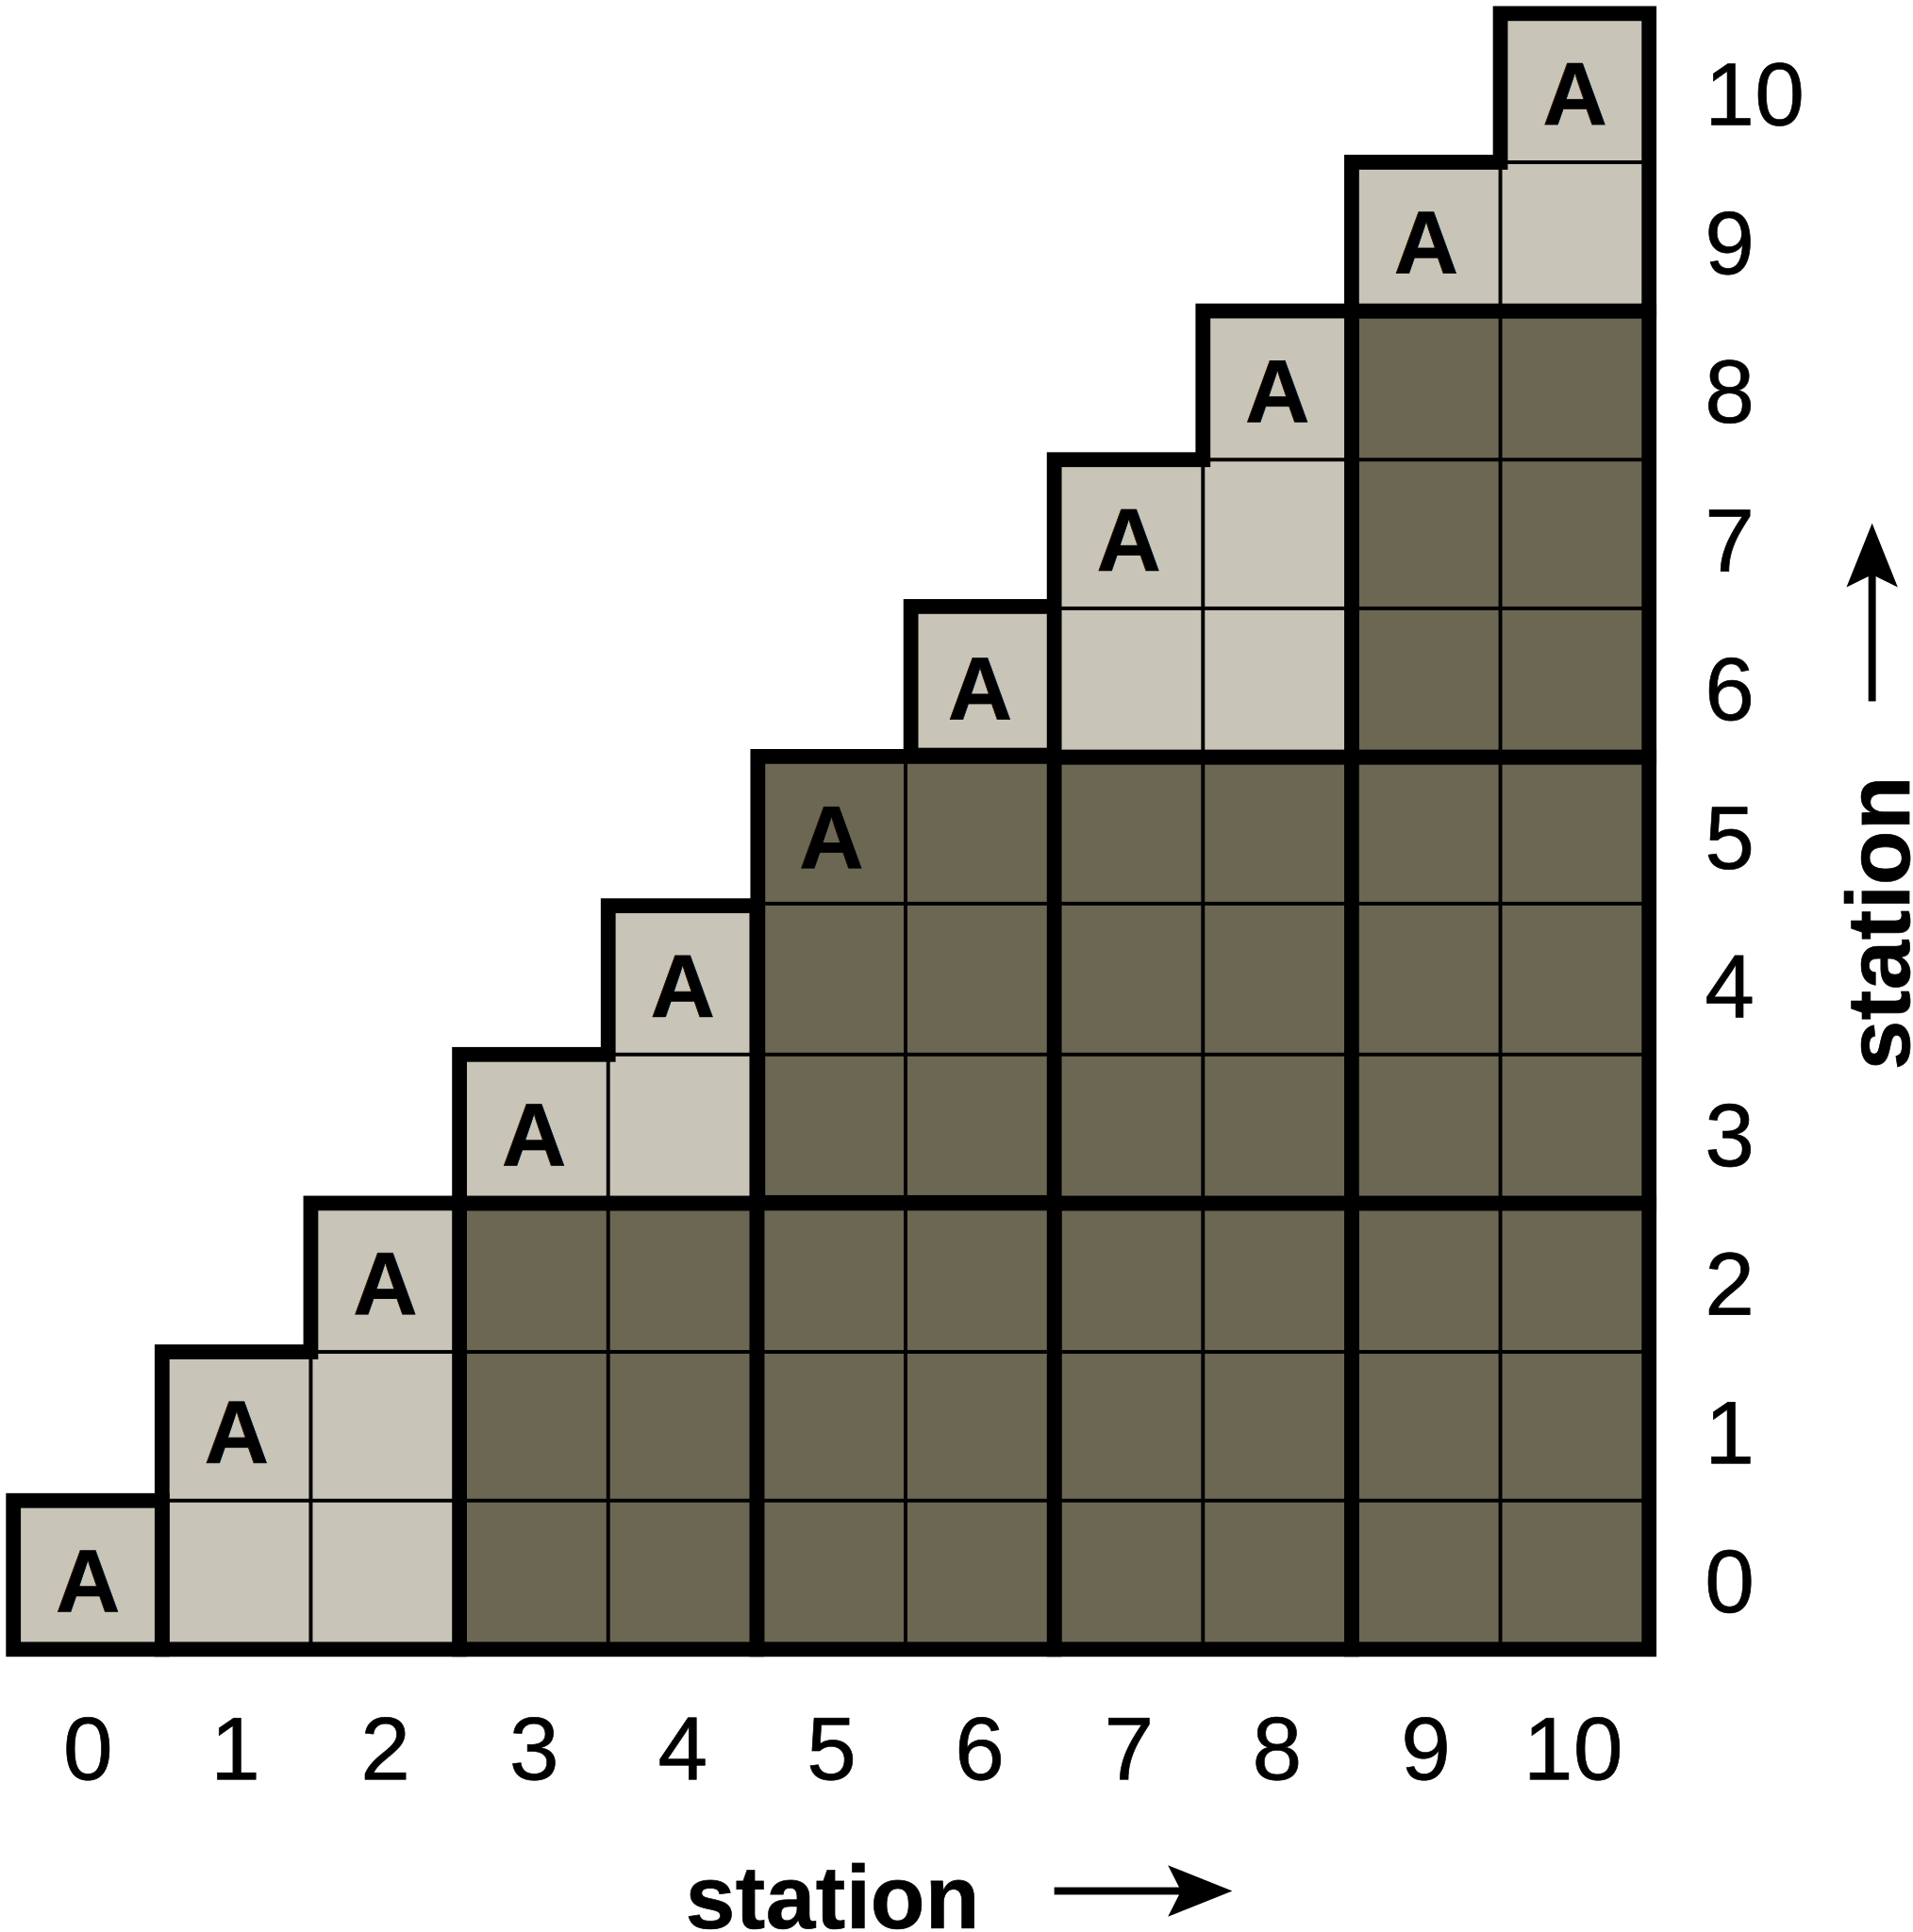
\includegraphics[width=4.2cm]{figures/correlation-triangle.pdf}
\end{center}
\vspace{-0.5cm}
\caption{An example correlation triangle.}
\label{fig-correlation}
\end{figure}

An important optimization that we implemented is the reduction
of memory loads by the correlator. 
A sample can be used multiple times by correlating it
with the samples from multiple other receivers in the same loop iteration.
For example, a sample from receiver A in the X polarization
that is loaded into a register pair can be correlated with the X and
Y polarizations of receivers B, C and D, using it six times. 
Figure~\ref{fig-correlation} shows how we correlate multiple
receivers at the same time. Each square represents the XX, XY,
YX, and YY correlations of the receivers as indicated by row and
column number. The figure is triangular, because we compute
the correlation of each pair of receivers only once. The squares labeled \emph{A} are
autocorrelations, which can be treated specially since they require only half
the amount of computations.
The triangle is divided into larger tiles, in this case 
2x3 tiles (the dark gray boxes), but arbitrary sizes are possible.
A tile is correlated as a unit. For example, the lower
right-hand-side rectangle correlates receivers 9 and 10 with receivers
0, 1, and 2.

It is important to tune the tile size to the architecture. We want to
make the tile size as large as possible, while still fitting in the
register file. This offers the highest level of data reuse.  
If we have a $w \times h$ tile size, the number of operations is given by $flops = 32wh$.
The number of bytes that has to loaded from memory is $16(w+h)$.
The minimum number of registers that is required is $4 (1 + min(w,h)) + 8 w h$.
This is the total number of registers, including accumulators, while reusing
registers if a value is no longer needed (hence the $min$ operation). However,
this formula does not count additional registers that could be needed for data prefetching,
address calculations and loop counters.
The number of registers is expressed in single-precision float registers. If an architecture has vector
registers, the result can be divided by the vector length.
Table~\ref{tile-size-table} shows the properties of different tile sizes. 

Despite the division of the correlation triangle in tiles, there
still is opportunity for additional data reuse \emph{between} tiles. 
The tiles
within a row or column in the triangle still need the same samples.
In
addition to registers, caches can thus also be used to increase data
reuse.  Since we know exactly what data can be reused at what moment, we
found it is important to have direct influence on the caches and the thread scheduler.  This
way, we can make sure that tiles in same row or column are calculated
at the same time by different threads. 
Because the algorithm is
extremely data intensive, the resulting optimized implementation on
many-cores is typically limited by the architecture's memory
bandwidth. The memory aspects of the algorithm are twofold.
There is an algorithmic part, the tile size, which is limited
by the number of registers. The second aspect is architectural in nature: the cache
sizes, cache hierarchy and hit ratio. Together, these two aspects dictate the
memory bandwidth that is needed to keep the ALUs busy.

\begin{table}
\begin{center}
{\small
\begin{tabular}{l|r|r|r|r}
tile & floating point & memory loads & arithmetic     &  minimum nr.           \\
size & operations     & (bytes)      & intensity      &  registers (floats)    \\
\hline
1x1  &  32            &   32         &   1.00         &  16                    \\
1x2  &  64            &   48         &   1.33         &  24                    \\
2x2  & 128            &   64         &   2.00         &  44                    \\
3x2  & 192            &   80         &   2.40         &  60                    \\
3x3  & 288            &   96         &   3.00         &  88                    \\
4x3  & 384            &  112         &   3.43         & 112                    \\
4x4  & 512            &  128         &   4.00         & 148                    \\
\end{tabular}
} %\small
\end{center}
\vspace{-0.5cm}
\caption{Properties of different tile sizes.}
\label{tile-size-table}
\end{table}

It is important to realize that the
correlator itself is \emph{trivially parallel}, since tens of thousands of
frequency channels can be processed independently.  This allows us to
efficiently exploit many-core hardware.

% naar metingen sectie
%We choose 64 as the number of receivers, since
%that is a realistic number for LOFAR.  Future instruments will likely
%have even more receivers. 


\subsection{Intel}
\subsection{BG/P}
\subsection{NVIDIA}
\subsection{ATI}
\subsection{Cell}


\section{Programmability}


\subsection{Aplying our techniques: a case study with the Intel Larrabee}

Intel recently disclosed some details about the upcoming Larrabee processor,
a fully programmable GPU based on the well-known x86 instruction set.
Although performance details are unknown, it is interesting to compare the
Larrabee to the aforementioned architectures, and to see how a correlator
should be implemented to obtain optimal performance.

The processing power comes from Larrabee's relatively long vector size:
a vector holds 16~elements, where the other architectures have vectors lengths
of at most~4.
The long vector size forces us to reconsider our parallelization strategy.
There are several options to perform 16~simultaneous FMAs.
One option is to operate on 16~samples with consecutive time stamps.
A minor drawback is that the data must be ``horizontally'' added to integrate,
but this can be done outside the main loop.
Another option is to operate on samples from 16~consecutive frequencies.
An advantage of this may be that the input is in the right order (i.e.,
the 16~values can be read from consecutive memory locations) if a Poly-Phase
Filter precedes the correlator: the FFT outputs consecutive frequencies into
consecutive memory locations.
Both 

Another option is to correlate samples from different receivers as illustrated
by Figure~\ref{fig:4x4-correlation}.
This method minimizes memory loads, but requires additional shuffling of data.
Unfortunately, the most efficient method can only be determined empirically,
when the hardware is available.

\section{Conclusions}


\bibliographystyle{IEEEbib}
\bibliography{spm}

\end{document}
